\section{Results}
All 144 planned evaluation runs completed. The trace audit reconciles 416 model calls and 568\,283 provider-reported tokens, including the 24-run skill ablation. There were 0 infrastructure or protocol execution errors; usage accounting is complete in every run. The six development-pilot runs are excluded. The preserved manifest and final hashes match, and the recorded order matches the frozen schedule.

Evaluation ran on 13 September 2026 from 13:09:45 to 13:33:34 UTC. This is an observed same-day API experiment, not a latency forecast for other accounts or deployments.

\begin{table}[htbp]
\centering\small
\setlength{\tabcolsep}{4pt}
\begin{tabular}{@{}lrrrrr@{}}
\toprule
\textbf{Condition} & \textbf{Strict} & \textbf{SQL norm.} & \textbf{Tokens/run} & \textbf{Mean s} & \textbf{Median s}\\
\midrule
Single agent & 20/24 & 23/24 & 1\,143 & 4.72 & 3.39\\
Sequential & 20/24 & 24/24 & 3\,410 & 13.72 & 11.77\\
Parallel & 19/24 & 23/24 & 3\,520 & 8.14 & 6.04\\
Hierarchical & 20/24 & 24/24 & 4\,373 & 11.19 & 10.01\\
Reflexive & 20/24 & 24/24 & 2\,714 & 9.77 & 6.26\\
\midrule
Hierarchical + all skills & 21/24 & 24/24 & 8\,518 & 11.93 & 10.88\\
\bottomrule
\end{tabular}
\caption{Observed results. Strict is the frozen primary score. SQL norm. is the explicitly post-hoc wrapper sensitivity; query text is unchanged. The separated last row is the skill-loading ablation.}
\label{tab:results}
\end{table}

\subsection{Format compliance and solution quality}
During evaluation, visible SQL answers exposed a distinction between a correct-looking query and the requested nested result shape. The primary grader was left unchanged. An explicitly post-hoc sensitivity wraps an existing raw string under answer as an object with a sql field, then executes the identical query against the same three fixtures. No SQL text, numeric answer, prompt or trial is repaired or repeated.

This normalization applies to 22 recorded outputs. It changes whole-task completions from 120/144 to 142/144 across the six conditions. The strict column measures delivered schema compliance as well as correctness; the normalized column diagnoses how much of the observed failure is attributable to that wrapper. It is not a second prespecified endpoint or proof that every generated query is correct outside these fixtures.

The two remaining failures are T05, repetition 2, under the single and parallel conditions. Both return a correct makespan of 38 but start H at 10 instead of 18 and K at 21 instead of 29. H depends on C finishing, and K depends on H finishing. This is a dependency-propagation error, not a JSON-wrapper error; checking only the final makespan would miss it.

\begin{figure}[htbp]
\centering
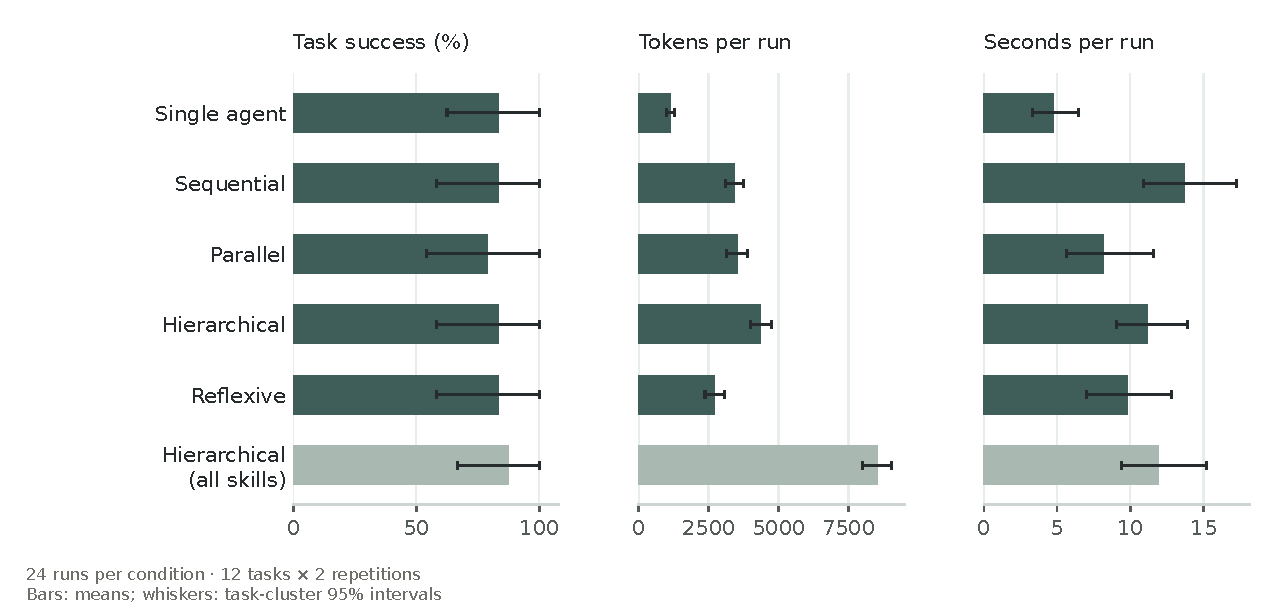
\includegraphics[width=\linewidth]{../../results/analysis/comparison-en.pdf}
\caption{Measured primary success, total tokens and elapsed time. Whiskers are descriptive 95\% task-cluster intervals. All-skills loading is shown separately. Figure generated from the released data.}
\label{fig:comparison}
\end{figure}

\subsection{Selected skills versus the complete catalog}
The hierarchical condition uses 4\,373 tokens per run on average with one selected skill, compared with 8\,518 when all ten bodies are loaded. The paired mean difference is 4\,145 tokens, with a 95\% interval [3898; 4366]. The increase is 94.8\%, interval [87.9; 101.9]\%.

Strict success changes from 20/24 to 21/24; under the wrapper sensitivity it changes from 24/24 to 24/24. The mean latency difference, all minus selected, is 0.74 seconds, interval [-0.24; 1.83]. This is a payload ablation with the correct family supplied in advance. It does not measure catalog-search errors or their token cost.

\subsection{Costs and uncertainty}
The reflexive workflow executes 5 revision calls across its 24 runs; a critic can add cost even when no revision follows. Provider-reported cached input totals 44\,788 tokens, and reported reasoning totals 97\,915. These are subsets, not additional tokens. Tables~\ref{tab:efficiency} and~\ref{tab:intervals} retain failed attempts and reflect the small number of independent task instances. Point rankings alone should not be interpreted as statistically established general superiority.

\begin{table}[htbp]
\centering\small
\setlength{\tabcolsep}{4pt}
\begin{tabular}{@{}lrrrr@{}}
\toprule
\textbf{Condition} & \textbf{Total tokens} & \textbf{Calls} & \textbf{Success/100k tok.} & \textbf{Success/min}\\
\midrule
Single agent & 27\,424 & 24 & 72.93 & 10.58\\
Sequential & 81\,845 & 72 & 24.44 & 3.64\\
Parallel & 84\,479 & 72 & 22.49 & 5.83\\
Hierarchical & 104\,963 & 95 & 19.05 & 4.47\\
Reflexive & 65\,133 & 58 & 30.71 & 5.12\\
\midrule
Hierarchical + all skills & 204\,439 & 95 & 10.27 & 4.40\\
\bottomrule
\end{tabular}
\caption{Resource efficiency using primary strict successes and all attempts. Accumulated successes/minute is not saturated-server throughput.}
\label{tab:efficiency}
\end{table}

\begin{figure}[htbp]
\centering
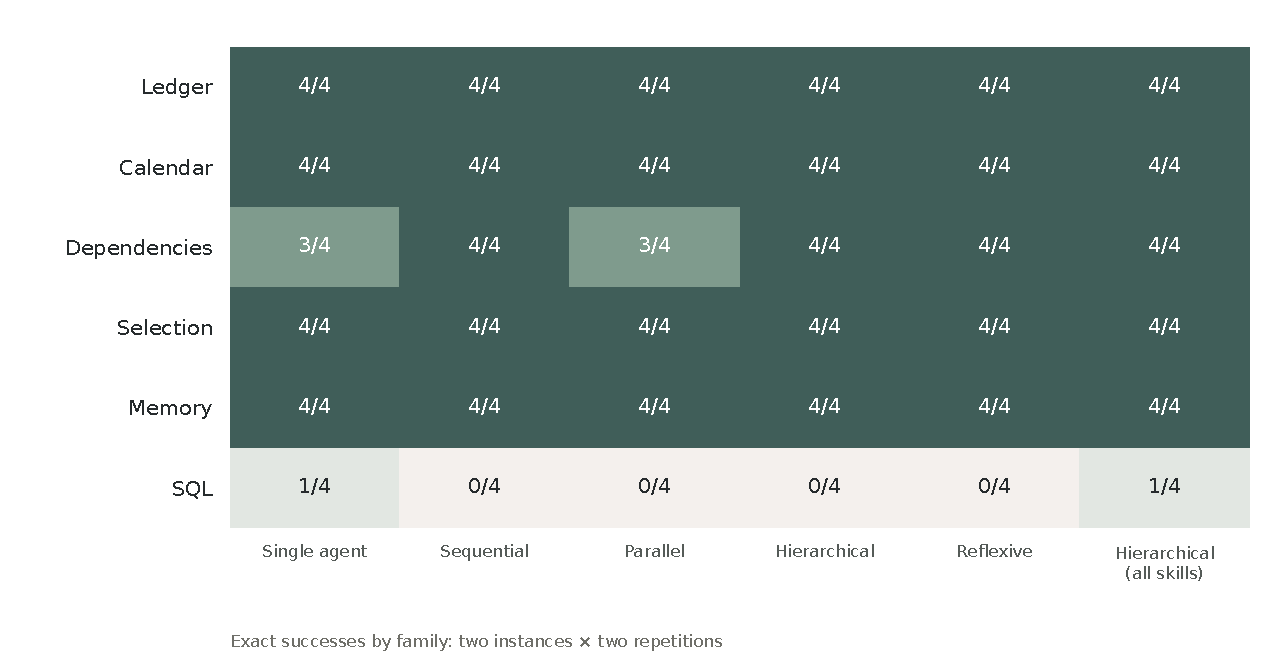
\includegraphics[width=\linewidth]{../../results/analysis/families-en.pdf}
\caption{Strict successes by task family. Each cell represents four runs, not four independent task instances. The SQL sensitivity is reported separately in Table~\ref{tab:results}.}
\label{fig:families}
\end{figure}

\begin{table}[htbp]
\centering\small
\setlength{\tabcolsep}{4pt}
\begin{tabular}{@{}lrrr@{}}
\toprule
\textbf{Condition} & \textbf{Success \%} & \textbf{Mean tokens} & \textbf{Mean seconds}\\
\midrule
Single agent & [62.5; 100.0] & [1005; 1279] & [3.33; 6.43]\\
Sequential & [58.3; 100.0] & [3094; 3752] & [10.90; 17.28]\\
Parallel & [54.2; 100.0] & [3157; 3904] & [5.65; 11.58]\\
Hierarchical & [58.3; 100.0] & [4012; 4740] & [9.04; 13.89]\\
Reflexive & [58.3; 100.0] & [2373; 3064] & [7.03; 12.82]\\
Hierarchical + all skills & [66.7; 100.0] & [7987; 9037] & [9.39; 15.22]\\
\bottomrule
\end{tabular}
\caption{Descriptive 95\% task-cluster bootstrap intervals for the primary metric, mean total tokens and mean wall time. Twelve task ids are the resampling units.}
\label{tab:intervals}
\end{table}
